\documentclass[aspectratio=1610]{beamer}

\usetheme{KTH}
\usepackage{caption}
\captionsetup[figure]{labelformat=empty}% redefines the caption setup of the figures environment in the beamer class.
\captionsetup[subfigure]{labelformat=empty}

\input{/home/peter/Organisatorisches/Latex_dinge/packages_beamer}

\addbibresource{/home/peter/EasterIslands/Literature/EasterIslandbib.bib}

\usepackage{appendixnumberbeamer}

\addtobeamertemplate{navigation symbols}{}{%
	\usebeamerfont{footline}%
	\usebeamercolor[fg]{footline}%
	\hspace{5em}%
	\insertframenumber/\inserttotalframenumber
}

\usepackage{mwe}

\usepackage{multimedia}
\usepackage{media9}

\author{Peter Steiglechner}
\title{Easter Island ABM}
\subtitle{Masterthesis Presentation Defence}
\institute{ZMT Bremen}
\date{\today}

% remove this if using XeLaTeX or LuaLaTeX
\usepackage[utf8]{inputenc}
\usepackage{wasysym}

\usepackage[ruled,vlined]{algorithm2e}

\AtBeginSection[]
{
	\begin{frame}[noframenumbering]{Outline}
	\begin{Large}\begin{center}
			\textbf{A Spatially Explicit Agent-Based Model \\ for Human-Resource Interaction on Easter Island}
	\end{center}\end{Large}
	\tableofcontents[currentsection]
\end{frame}
}

\begin{document}
	
	\startpage
	%%%%%%%%%%%%%%%%%%%%%%%%%%%%%%%%%%%%%%%%%%%%%%%%%%%%%%%%%%%%
	\begin{frame}[noframenumbering]
	
	\vspace{0.02\textheight}
	\begin{Large}\begin{center}
		\textbf{A Spatially Explicit Agent-Based Model \\ for Human-Resource Interaction on Easter Island}
\end{center}\end{Large}
	\vspace{0.01\textheight}

	\begin{small}
		\begin{center}
		En Rumsligt Explicit Agentbaserad Modell av Interaktionen mellan Människor och Resurser på Påskön
		\end{center}

	\end{small}
	
	\vspace{0.02\textheight}
	
	\begin{small}
		\begin{center}
		\textit{Peter Steiglechner, 29 June 2020}
		\end{center}

	\end{small}
\end{frame}


\normalpage


\begin{frame}[noframenumbering]
\frametitle{Outline}
	\begin{Large}\begin{center}
	\textbf{A Spatially Explicit Agent-Based Model \\ for Human-Resource Interaction on Easter Island}
	\end{center}\end{Large}
\tableofcontents
\end{frame}



\section{Easter Island History}
% !TEX root = presentation_29Jun.tex


\begin{frame}{Easter Island Mystery}
	\centering
	\begin{columns}
		\begin{column}{0.7\textwidth}
				\includegraphics[width=\linewidth]{../../EIMap_Merico2017}
			\captionof{figure}{\citet{Merico2017}}
		\end{column}
	\pause\begin{column}{0.3\textwidth}
	\centering
	\includegraphics[width=0.7\linewidth]{../../Diamond2011Cover}
	\captionof{figure}{\citet{Diamond2011}}
	\end{column}
	\end{columns}
\end{frame}

\begin{frame}{Facts of Easter Island History}
\centering
%\begin{itemize}
%	\item Forest
%	\item Polynesian Rats
%	\item Intensified deforestation from $1200\, {\rm A.D.}$ in many locations
%	\item Intensified farming (with the use of lithic mulching)
%	\item Moai statues carved between $1200$ and $1700 \, {\rm A.D.}$
%	\item European voyages arrive in $1722$, $1770$s, ... and introduce European diseases and slave trade (especially in the 19th century)
%\end{itemize}
%But: Pollen and Charcoal data is scarce and difficult to interpret.
\begin{figure}
	\centering
	\begin{subfigure}{0.15\textwidth}
	\centering
	\only<1-6>{\includegraphics[height=1cm]{images/ForestGerdCloseRull2020.jpg}
	\caption{{\scriptsize Palm Forest }}}
	\end{subfigure}\hfill
	\begin{subfigure}{0.15\textwidth}
	\centering
	\only<1-6>{	\includegraphics[height=1cm]{images/Rapa-Nui-Landscape.jpg}
	\caption{{\scriptsize Deforestation}}}
	\end{subfigure}\hfill
	\begin{subfigure}{0.15\textwidth}
	\centering
	\only<1-6>{	\includegraphics[height=1cm]{images/Pacific_rat.jpg}
		\caption{{\scriptsize Pacific Rats}}}
	\end{subfigure}\hfill
	\begin{subfigure}{0.15\textwidth}
	\centering
	\only<1-6>{\includegraphics[height=1cm]{images/lithicMulching.jpg}
	\caption{{\scriptsize Agriculture}}}
	\end{subfigure}\hfill
	\begin{subfigure}{0.15\textwidth}
	\centering
	\only<1-6>{	\includegraphics[height=1cm]{images/moai3.jpg}
	\caption{{\scriptsize Moai Statues}}}
	\end{subfigure}\hfill
	\begin{subfigure}{0.18\textwidth}
	\centering			\only<1-6>{\includegraphics[height=1cm]{images/voyages.png}
	\caption{{\scriptsize European Contact}}}
	\end{subfigure}
\end{figure}
%
\begin{figure}
	\centering
	\only<1>{\includegraphics[height=4cm]{images/ForestGerdCloseRull2020.jpg}
	\caption{Palm Forest}
	\flushright{\tiny Artisitc Rendering, \citet{Rull2020}}
	}	
	\only<2>{\includegraphics[height=4cm]{images/Rapa-Nui-Landscape.jpg}
	\caption{Deforestation}
	\flushright{\tiny Modern Day Image \url{en.wikipedia.org/wiki/Easter_Island}}
	}
	\only<3>{\includegraphics[height=4cm]{images/Pacific_rat.jpg}
	\caption{Pacfic Rats}
	\flushright{\tiny \url{de.wikipedia.org/wiki/Pazifische_Ratte}}
	}
	\only<4>{\includegraphics[height=4cm]{images/lithicMulching.jpg}
		\caption{Agriculture}
		 	\flushright{\tiny \citet{Hunt2009}}}
	\only<5>{\includegraphics[height=4cm]{images/moai3.jpg}
		\caption{Moai Statues}
	\flushright{\tiny \url{https://nl.wikipedia.org/wiki/Moai}}
	}
	\only<6>{
		\begin{columns}
			\centering
			\begin{column}{0.4\textwidth}
				\includegraphics[height=4cm]{images/voyages.png}
				\caption{European Contact}
			\end{column}
			\begin{column}{0.4\textwidth}
			
				\textbf{Observations:} \vspace{0.2cm}
%				\begin{columns}
%					\begin{column}{0.3\textwidth}
%						\begin{itemize}
%							\item Advanced civilisation 
%							\item Initially Dense Forest
%						\end{itemize}
%					\end{column}
%					\begin{column}{0.1\textwidth}\centering
%						\textbf{\Huge \lightning}
%					\end{column}
%					\begin{column}{0.6\textwidth}
%						\begin{itemize}
%							\item Declining population number, 
%							\item Moai on the floor, 
%							\item Barren Island
%						\end{itemize}
%				\end{column}
%				\end{columns}
			\begin{itemize}
				\item Advanced civilisation 
				\item Initially dense forest
				\item Barren island
				\item Declining population number
				\item Moai lying on the ground
			\end{itemize}
			\end{column}
		\end{columns}
	\flushleft{\tiny  \url{www.nytimes.com/2017/10/12/science/easter-island-dna-south-america.html}}
	}

		
%	\only<7>{\centering \textbf{Observations}\begin{columns}
%			\begin{column}{0.4\textwidth}
%				\begin{itemize}
%					\item Dense Forest before human arrival
%					\item Built Moai Statues
%					\item Used Advanced farming techniques
%				\end{itemize}
%			\end{column}
%		\begin{column}{0.05\textwidth}
%			\centering
%			{\Huge\lightning}
%		\end{column}
%			\begin{column}{0.4\textwidth}
%				\begin{itemize}
%					\item Only a few thousand people ($100$ in $1860\, {\rm A.D.}$) 
%					\item Moai Statues on the floor
%					\item  Barren Island (no large vegetation)
%				\end{itemize}
%				
%			\end				\end{columns}{column}
%		\end{columns}}
\end{figure}
\begin{figure}
	\centering

\only<1-3>{\includegraphics[width=0.6\linewidth]{images/timeline}}
\only<4,5>{\includegraphics[width=0.6\linewidth]{images/timeline_agric}}	\only<6>{\includegraphics[width=0.6\linewidth]{images/timeline_european}}
\end{figure}
\end{frame}

\begin{frame}{The Mystery -- Two Major Narratives}
\begin{columns}
		\begin{column}{0.4\textwidth}
		\textbf{Ecocidal View}\\ \citet{Brander1998}, \citet{Diamond2011}, \citet{Bahn2017} \\ \ \\
		Early arrival, \\ 
		\ra Population grows slowly exponentially, \\
		\ra Intensification of agriculture and deforestation, \\
		\ra Population reaches $6k$ to $20k$ people in 17th century, \\ 
		\ra Overexploitation of resources and conflict (Malthusian catastrophe),
		\\
		\ra `Collapse' prior to European contact
	\end{column}


	\begin{column}{0.4\textwidth}
		\textbf{Genocidal View}\\ \citet{Peiser2005}, \citet{Hunt2007}, \citet{Basener2008}\\ \  \\
		Late arrival, \\
		\ra Population grows quickly and then remains constant at $4k$ people, \\
		\ \\
		\ra Rats cause deforestation, \\
		\ra Humans resilient, \\
		 \ \\
		\ra European contact triggers decline due to slave trades and diseases \\
		 \ \\
		 \ \\
		 

	\end{column}

\end{columns}
\centering
{\color{red}$\Downarrow$}\\
{\color{red} Population dynamics?}
\end{frame}


%
%\begin{frame}{The Mystery -- Two Narratives}
%\begin{columns}
%	\begin{column}{0.2\textwidth}
%		\ \\ \ \\ \ \\
%		\begin{itemize}
%			\item Arrival
%			\item Growth of Human Population
%			\item Deforestation
%			\item Agriculture intesification
%			\item Population size peak
%			\item Aftermath
%		\end{itemize}
%	\end{column}
%	\begin{column}{0.4\textwidth}
%		\textbf{Genocidal View}\\ \citet{Hunt2007} \\ \ 
%		\begin{itemize}
%			\item $1200\, {\rm A.D.}$
%			\item Fast 
%			\item Because rat population sky-rockets
%			\item immediately, after $1200\, {\rm A.D.}$
%			\item at $4$ k people in $14th century$
%			\item Civilisation resilient to environmental degradation, but `genocide' due to European diseases and slave trade
%		\end{itemize}
%	\end{column}
%	\begin{column}{0.4\textwidth}
%		\textbf{Ecocidal View}\\ \citet{Diamond2011}, \citet{Bahn2017}, \citet{Brander1998}
%		\begin{itemize}
%			\item before $1000\,{\rm A.D.}$
%			\item Slow
%			\item Humans started deforesting and lived off the natural resources (provided by trees)
%			\item only after $1200\, {\rm A.D.}$
%			\item at $6-20$ k people in $17$th century
%			\item Overexploitation and erosion, resources scarce, potential conflict, `collapse' (Malthusian Catastrophe) prior to European contact
%		\end{itemize}
%	\end{column}
%\end{columns}
%\end{frame}


\section{Traditional Approach: Dynamic System Modelling}
% !TEX root = presentation_29Jun.tex

\begin{frame}{Mathematical Modelling of Human-Resource Interaction}

\begin{itemize}
	\item Macroscopic variables: 
	\begin{itemize}
		\item Resource stock (palm trees): $T$
		\item Human population size: $P$
	\end{itemize} 
	\ra Human-resource interactions (Lotka-Voltera predator-prey type)
	\item So far: Dynamics described by ordinary differential equations (ODEs)
	\begin{eqnarray*}\label{eq:ode}
		\frac{d \text{P}}{dt} & = & r_\text{P} (\text{T, P, H}(\text{P})) \ \cdot \ \text{P} \\
		\frac{d \text{T}}{dt} & = & r_\text{T} (\text{T}) \ \cdot \ \text{T} \ - \   \text{H}(\text{P}) 
	\end{eqnarray*}	
with \center{$\text{H}(\text{P})$ = harvest of population $\text{P}$; \\$r_{\rm T,P}$ = functions for rates of growth}
\end{itemize}
\end{frame}

\begin{frame}{The first model on Easter Island: \citet{Brander1998}}
%The first Model: \citeTitle{Brander1998}
\centering

%\item Population grows/decays exponentially. Consumption of the resource increases the rate
%\item Result: Slow regrowth of the palm tree vs.\ faster exponential population growth \ra Malthusian Catastrophe (a.k.a.\ `Boom-Bust')

\begin{columns} \begin{column}{0.7\textwidth}
		\includegraphics[width=\textwidth]{../../Thesis/images/Brander1998_EIBaseCase_presentation} 
\end{column}
\begin{column}{0.2\textwidth}
	{\footnotesize Model by \citet{Brander1998}}
\end{column}
\end{columns}
	

\begin{itemize}
\pause\item Extensions:
\begin{itemize}
	\item Socio-economic institutions \citep{Good2006}
	\item Second resource \citep{DAlessandro2007}
	\item Rat population \citep{Basener2008}
	%\item 1-dim spatial component \citep{Basener2011}
	\item Disease model \citep{Brandt2015}
\end{itemize} 
\end{itemize}                                                       
\end{frame}

\begin{frame}{Shortcomings of Dynamic System Models}
\begin{itemize}
\item Uncertainty in Parameters\\ \vspace{0.3cm}
{\centering 
	\begin{columns}
		\begin{column}{0.7\textwidth}
			\includegraphics[width=\textwidth]{../../Brandt2015_onlyHumans}
		\end{column}
		\begin{column}{0.15\textwidth}
			{\footnotesize Model by \citet{Brandt2015}}
		\end{column}
	\end{columns}
} \vspace{0.3cm}
\ra Macroscopic view does not give insight into plausibility of resulting trajectory
\pause\item Neglect ...
\begin{itemize}
\item Spatial constraints
\item Irreducibility and heterogeneity
\item Adaptation and emergent phenomena
\item Stochasticity
\end{itemize} 
\vfill 
{\tiny More in e.g.\ \citet{Bookstaber2019}, \citet{Bonabeau2002}}
\end{itemize}
\end{frame}



\section{New Approach: Agent-Based Modelling (ABM)}
% !TEX root = presentation_29Jun.tex

%\begin{frame}{Agent Based Modelling}
%\end{frame}
%
%\begin{frame}{Modelling Societies with ABM}
%
%%\begin{block}{\citet{Bookstaber2019}}
%%	\TODO
%%\end{block}
%\end{frame}


\begin{frame}{What is Agent-Based Modeling (ABM)}
%\begin{itemize}
%	\item Discrete units (Agents) in an environment with specific traits
%	\item Asynchronous and autonomous update of agents:
%	%\item In each update: 
%	\begin{itemize}
%		\item interaction based on rules and heuristics \\(often non-linear, heterogeneous, stochastic, adaptive, path-dependent)
%		\item autonomous decisions of agents
%	\end{itemize}
%	\item Aggregate variables are (1) outcomes of and (2) contexts for the agents decisions and actions \citep{Kohler2000}
%\end{itemize}



\begin{algorithm}[H]
	\textbf{Initialise} Environment  \\
	\textbf{Initialise} discrete Agents with specific traits in some location within the environment\\
	\For{$t \ \in\  \{t_{\rm start}, t_{\rm end}\}$}{
		\For{agent (in asynchronous order)}{
			\textbf{Interaction} between agent and environment based on rules and heuristics\\
			\textbf{Update} agent according to autonomous decisions
		}
		\textbf{Calculate} aggregate variables of environment and agents
	}
	\caption{General Structure}
\end{algorithm}
\end{frame}



\begin{frame}{Advantages of ABM with respect to ODE models}


% 	\begin{block}{\citet{Epstein1996}}%, as cited in \citet{Bonabeau2002}}
% 		 \begin{framed}
%	On Agent-Based Modelling:
%	"Perhaps one day people will interpret the question, ‘Can you explain [an observed social phenomenon]?’ as asking `Can you grow it?’"
%\end{framed}
%	 	\end{block}
 	 	%, as cited in \citet{Bonabeau2002}}
 	 	\begin{framed}
 	 		 \citet{Epstein1996}, \citet{Bonabeau2002} on Agent-Based Modelling:
 			\begin{center}
 				\textit{"Perhaps one day people will interpret the question, ‘Can you explain [an observed social phenomenon]?’ as asking `Can you grow it?’"
} 			\end{center}
 		\end{framed}

	From macroscopic, top-down description \ra to microscopic, bottom-up description
	\begin{enumerate}
		\item ABM allows for rules and heuristics to be 
		\begin{itemize}
			\item non-linear, discontinuous
			\item heterogeneous,
			\item stochastic, 
			\item adaptive \newline
			%\item path-dependent 
			\ra non-ergodicity \& computational irreducibility
		\end{itemize}
		\pause\item \ra Emergent phenomena
		%\item Non Ergodicity
		%\pause\item \ra Computational irreducibility
		\pause\item Decisions include stochasticity
		\pause\item Natural implementation of heterogeneous space dependency
	\end{enumerate}
\end{frame}


%\begin{frame}{Application of ABMs}
%\begin{itemize}
%	\item Typically: Problems related to cognitive psychology, game theory, and complexity science \citep{Bousquet2004}
%	\item Also, Socio-ecological Systems \citep{Muller-Hansen2017} \ra Human-Resource Interaction
%	\begin{itemize}
%		\item \ldots
%		\item Collapse of Ancient Societies
%		\begin{itemize}
%			\item Anasazi in Arizona, US \citet{Axtell2002}
%			\item Maya \citet{Heckbert2013}
%			\item Now: Easter Island
%		\end{itemize}
%	\end{itemize}
%\end{itemize}
%\end{frame}



\section{The Easter Island ABM}
% !TEX root = presentation_29Jun.tex


\begin{frame}{Easter Island ABM -- Overview}  
%\begin{overlayarea}{\textwidth}{\textheight} 
\begin{itemize}
	\item<2-> Agents (dots) are households of a few dozen (ca.\ up to $40$) individuals.
	\item<3-> Environment provides trees and farming products
	\item<3-> Agents harvest from local environment (cut trees and occupy farming sites)
	\item<4-> If successful, the agent's population grows (eventually producing more agents) \newline If not successful, it decreases and the agent moves
	\item<5-> Agents adapt their resource preference according to the perceived local environment
\end{itemize}%
	\centering
	\includegraphics[width=0.7\linewidth]{images/map_time1600}
	%\captionof{figure}{Example Snapshot}
%\end{overlayarea}
\end{frame}

\begin{frame}{Create the Environment -- Discretisation}
	\centering
	\includegraphics[width=0.7\linewidth]{images/Plot_elevation}


\end{frame}

\begin{frame}{Create the Environment -- Features}
\centering
\only<1>{\includegraphics[width=0.7\linewidth]{../../Thesis/images/SketchABM2/EnvironmentSketch_1}}
\only<2>{\includegraphics[width=0.7\linewidth]{../../Thesis/images/SketchABM2/EnvironmentSketch_2}}
\only<3>{\includegraphics[width=0.7\linewidth]{images/map_carrCap}
\captionof{figure}{Based on \citet{Mieth2015}, \citet{Bahn2017}, \citet{Rull2020}}
}
\only<4>{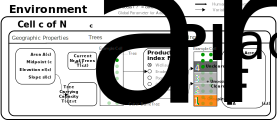
\includegraphics[width=0.7\linewidth]{../../Thesis/images/SketchABM2/EnvironmentSketch_final}
	\captionof{figure}{$1\, {\rm acre} \ \hat{\approx} \ 100\, {\rm m} \, \times 40\,{\rm m}$.}}
\only<5>{\includegraphics[width=0.7\linewidth]{images/Plot_F_PI_c}
	\captionof{figure}{Based on \citet{Louwagie2006}, \citet{Puleston2017}}}
\end{frame}

\begin{frame}{Agents and Interaction with Environment}
\centering
\only<1>{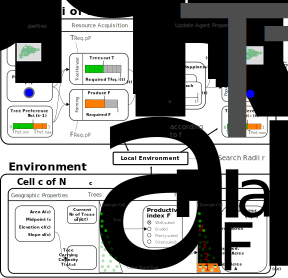
\includegraphics[width=0.55\linewidth]{../../Thesis/images/SketchABM2/sketch_triangles}}
%\only<2>{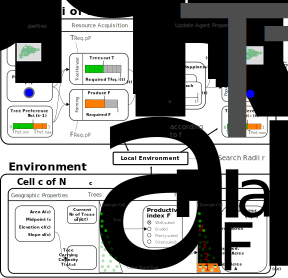
\includegraphics[width=0.85\linewidth]{../../Thesis/images/SketchABM2/sketch_triangles}}
\only<2>{\includegraphics[width=0.85\linewidth]{../../Thesis/images/SketchABM2/Agent_Props}}
\only<3>{\includegraphics[width=0.85\linewidth]{../../Thesis/images/SketchABM2/Agent_Harvest}}
\only<4>{\includegraphics[width=0.85\linewidth]{../../Thesis/images/SketchABM2/Agent_Update2}}
\only<5>{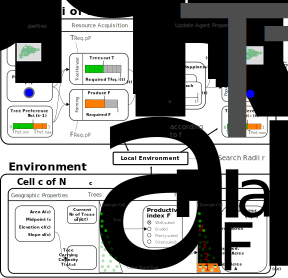
\includegraphics[width=0.85\linewidth]{../../Thesis/images/SketchABM2/sketch_triangles}}
\end{frame}

%\begin{frame}
%Exceptions: Fishing.
%\end{frame}


\begin{frame}{Moving: Decision Making based on Penalties}

\begin{columns}
\begin{column}{0.2\textwidth}
	\centering
	\only<1>{\includegraphics[height=2cm]{images/white}\captionof{figure}{\scriptsize \ \  }}
	\only<2->{\includegraphics[height=2cm]{../../Thesis/images/Results/Standard/Penalties_AG500_t=1603_G}
	\captionof{figure}{\scriptsize Geography}}
\end{column}%\hfill
\begin{column}{0.2\textwidth}
	\centering
	\only<3->{\includegraphics[height=2cm]{../../Thesis/images/Results/Standard/Penalties_AG500_t=1603_W}
	\captionof{figure}{\scriptsize Water}}
\end{column} 
\begin{column}{0.2\textwidth}
\centering
\only<4->{\includegraphics[height=2cm]{../../Thesis/images/Results/Standard/Penalties_AG500_t=1603_D}
	\captionof{figure}{\scriptsize Pop.\ Density}}
\end{column}
\begin{column}{0.2\textwidth}
\centering
\only<5->{\includegraphics[height=2cm]{../../Thesis/images/Results/Standard/Penalties_AG500_t=1603_T}
	\captionof{figure}{\scriptsize Trees}}
\end{column}
\begin{column}{0.19\textwidth}
\centering
\only<6->{\includegraphics[height=2cm]{../../Thesis/images/Results/Standard/Penalties_AG500_t=1603_F}
	\captionof{figure}{\scriptsize Farming Sites}}
\end{column}
\end{columns}

\vfill
\centering
\begin{columns}
	\begin{column}{0.35\textwidth}
		\includegraphics[height=4.5cm]{../../Thesis/images/Results/Standard/Penalties_AG500_t=1603_Situation}
	\end{column}
	\begin{column}[t]{0.25\textwidth}
	 	\only<2>{\textbf{Avoid cells...\\ ...
	  	with large elevation and large slope}}%
  		\only<3>{\textbf{Avoid cells...\\ ...
  				far from a (big) freshwater source   }}%
  		\only<4>{\textbf{Avoid cells...\\ ...
  				in regions with large population density}}%	
 			\only<5>{\textbf{Avoid cells...\\...
 					with few trees nearby  }}%
				\only<6>{\textbf{Avoid cells... \\ ...
						with few (well-suited) available farming sites nearby}}%
  		\only<7>{\textbf{\begin{center} {\Huge$\Downarrow$} \end{center} \ra \quad Total\quad \ra }}
  	
	\end{column}
	\begin{column}{0.35\textwidth}
		\only<2>{\includegraphics[height=4.5cm]{../../Thesis/images/Results/Standard/Penalties_AG500_t=1603_G}}%
		\only<3>{\includegraphics[height=4.5cm]{../../Thesis/images/Results/Standard/Penalties_AG500_t=1603_W}}%
		\only<4>{\includegraphics[height=4.5cm]{../../Thesis/images/Results/Standard/Penalties_AG500_t=1603_D}}%	
		\only<5>{\includegraphics[height=4.5cm]{../../Thesis/images/Results/Standard/Penalties_AG500_t=1603_T}}%	
		\only<6>{\includegraphics[height=4.5cm]{../../Thesis/images/Results/Standard/Penalties_AG500_t=1603_F}}%
		\only<7>{\includegraphics[height=4.5cm]{../../Thesis/images/Results/Standard/Penalties_AG500_t=1603_tot}}
	\end{column}
\end{columns}
%

\end{frame}


\begin{frame}{The Full Model}
\begin{columns}
	\column[T]{0.69\textwidth}
		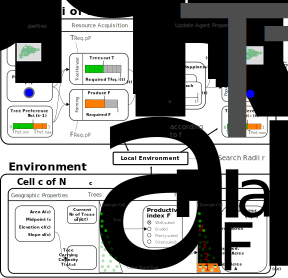
\includegraphics[height=0.85\textheight]{../../Thesis/images/SketchABM2/sketch_triangles}
	\column[T]{0.29\textwidth}
		\includegraphics[height=3.5cm]{../../Thesis/images/Results/Standard/Penalties_AG500_t=1603_tot}
\end{columns}
\end{frame}
	




\section{Results and Discussion}
% !TEX root=frame_thesis.tex
\section{Results and Discussion}



\begin{frame}{Conclusions}
\begin{itemize}
	\pause\item Limits of the study:
	\begin{itemize}
		\item Rules and processes often based on plausibility arguments
		\item Uncertainty in the available data
		\item More complex than macroscopic ODE models.
		\item Possible improvements of the model
		\begin{itemize}
			\item Social structure
			\item From myopic to far-sighted, sustainable harvest behaviour of agents
			\item Stochasticity and uncertainty in the harvest behaviour of agents
		\end{itemize}
	\end{itemize}
	\vspace{1cm}
	\pause\item Benefits of the Model:
	\begin{itemize}
		\item Change of perspective on Easter Island: \newline From macroscopic, top-down to microscopic, bottom-up
		\item Spatial considerations
		\item Identifying regions of interest for archaeological work \& \newline Interpret data from single locations
	\end{itemize}
\end{itemize}
\end{frame}


\begin{frame}[noframenumbering]{Summary}
\begin{Large}\begin{center}
		\textbf{A Spatially Explicit Agent-Based Model \\ for Human-Resource Interaction on Easter Island}
\end{center}\end{Large}
\begin{minipage}[t][0.66\textheight][t]{0.6\textwidth}
	\vspace{0pt}
	\tableofcontents
\end{minipage}
\begin{minipage}[t][0.7\textheight][t]{0.35\textwidth}
	\vspace{0pt}
		\includegraphics[width=\linewidth]{images/summaryEI}
	\includegraphics[width=0.7\textwidth]{../../Thesis/images/Brander1998_EIBaseCase_presentation}
	\includegraphics[width=0.8\linewidth]{images/map_time1500}
\end{minipage}
%\end{columns}

\end{frame}

\begin{frame}{Thank you!}

\vspace{0.02\textheight}

\begin{Large}
	A Spatially Explicit Agent-Based Model for Human-Resource Interaction on Easter Island
\end{Large}

\vspace{0.02\textheight}
\centering
\includegraphics[width=0.5\linewidth]{images/map_time1500}
% \movie[width=0.6\textwidth, showcontrols=true, poster, autostart]{\includegraphics[width=0.6\textwidth]{images/map_time800}}{movieFast.mp4}
% 
% \includemedia[
% width=0.6\textwidth,height=0.6\textheight,
% activate=pageopen,
% addresource=movieFast.mp4,
% flashvars={
% 	source=movieFast.mp4
% 	&autoPlay=true
% }
% ]{}{VPlayer.swf}
 
 \vfill 
Special thanks to Agostino Merico, Esteban Acevedo Trejos, and Michael Hanke.

\end{frame}


\appendix
% !TEX root = presentation_29Jun.tex



\section{Backup}
\subsection{Methods}
\begin{frame}{Burning and Occupying Land}
	\centering
	\includegraphics[width=0.7\linewidth]{../../Thesis/images/SketchABM2/burningSketch_triangle}
\end{frame}

\begin{frame}{Different Tree Preference Strategies}
	\centering
\includegraphics[width=0.7\linewidth]{../../Thesis/images/TPref}
\end{frame}

\begin{frame}{Population Growth Function}
\centering
\includegraphics[width=0.7\linewidth]{../../Thesis/images/populationchange_g}
\end{frame}

\subsection{More Results}


\begin{frame}{Movie}
\movie[width=\textwidth, showcontrols=true, poster]{\includegraphics[width=\textwidth]{images/map_time800}}{movieFast.mp4}
%\includemedia[
%width=0.7\textwidth,height=6cm,
%activate=pageopen,
%addresource=movieFast.mp4,
%flashvars={
%	source=movieFast.mp4
%	&autoPlay=true
%}
%]{}{VPlayer.swf}
\end{frame}



\begin{frame}{Result 1: Spatio Temporal}
\centering
\includegraphics[width=0.6\linewidth]{../../Thesis/images/Results/Standard/EnsembleStatistics+Panels}
\end{frame}


\begin{frame}{Clustering}
	\centering
	\includegraphics[width=0.7\linewidth]{../../Thesis/images/ClusterSTDS1650}
\end{frame}


\begin{frame}{Ensemble: Realisations}
	\centering
	\includegraphics[width=0.7\linewidth]{../../Thesis/images/RealisationsOfPopGrowth}
\end{frame}

\begin{frame}{Ensemble: Coefficient of Variation}
	\centering
	\includegraphics[width=0.7\linewidth]{../../Thesis/images/Results/Standard/CoeffOfVariation}
\end{frame}

\begin{frame}{Indicators: Acceleration and Collapse Phase}
\centering
\includegraphics[width=0.7\linewidth]{../../Thesis/images/Results/Standard/StandardsecondaryStats}
\end{frame}



\begin{frame}{Net Growth Rate}
	\centering
	\includegraphics[width=0.7\linewidth]{../../Thesis/images/Results/Standard/NetGrowthRate}
\end{frame}


\subsection{Larger and Smaller T Req}

\begin{frame}
	\centering
	\includegraphics[width=\linewidth]{../../Thesis/images/Results/EnsembleStatistics_largersmallerRad}
\end{frame}





\subsection{Moving Results}
\begin{frame}{Optimal Location}
	\centering
	\includegraphics[width=0.5\linewidth]{../../Thesis/images/Results/Moving/alphaDeterministic_EnsembleStatistics+Panels}
\end{frame}
\begin{frame}{Trial and Error Hopping}
	\centering
	\includegraphics[width=0.5\linewidth]{../../Thesis/images/Results/Moving/alphaHopping_EnsembleStatistics+Panels}
\end{frame}
\begin{frame}{Resources Only}
	\centering
	\includegraphics[width=0.5\linewidth]{../../Thesis/images/Results/Moving/alphaResource_EnsembleStatistics+Panels}
\end{frame}



\end{document}
%%%%%%%%%%%%%%%%%%%%%%%%%%%%%%%%%%%%%%%%%%%%%%%%%%%%%%%%%%%%
%\begin{frame}
%\frametitle{Making a KTH Presentation}
%
%\begin{block}{Steps needed}
%	\begin{itemize}
%		\item Copy the following files:
%		\begin{itemize}
%			\item \texttt{examplepresentation.tex} (this file)
%			\item \texttt{beamerthemeKTH.sty}
%			\item \texttt{kthgraphics} (with all its contents)
%		\end{itemize}
%		\item Replace the contents in \texttt{examplepresentation.tex} with your own
%		\item Run \texttt{pdflatex} (or \texttt{xelatex} or \texttt{lualatex}) a couple of times
%		\item Present your slides using a PDF-viewer
%	\end{itemize}
%\end{block}
%
%\end{frame}
%
%\end{document}


%
%
%\section{Introduction}
%%\subsection{The mystery of the Easter Island society}
%\input{EasterIslandHistory}
%%\subsection{Modelling answers to the mystery}
%\input{EImodels}
%%\subsection{Agent Based Modelling}
%\input{ABMintro}
%
%\section{Methods/Model}
%%\subsection{General Idea}
%\input{GeneralEIABM}
%%\subsection{Modules}
%%\subsubsection{Harvest -- Trees and Agriculture}
%%\subsubsection{Moving}
%%\subsubsection{Reproduction and Death}
%%\subsection{Statistical Runs}
%\section{Results}
%\input{Results}
%
%\end{document}